\chapter{Esperimenti e risultati}
\label{chap:esperimenti}


% ...
%  - metodo, obiettivi, metriche, ambiente\&strumenti
 
% La metrica utilizzata per valutare i modelli è l'accuratezza, misurata sui dati di test. 
% ...


% Tutti gli esperimenti sono stati eseguiti su un server con CPU Intel(R) Xeon(R) W-1250P CPU @ 4.10GHz e con 31GB di ram. Il linguaggio di programmazione utilizzato è Python 3.10.10 ed è stato utilizzato il risolutore Gurobi 10.0.1~\cite{gurobi}. 

\section{Dataset}
% Nel valutare algoritmi di addestramento automatico, è di fondamentale importanza la scelta dei dataset utilizzati, dato che l'apprendimento è basato proprio su di essi. 
% Per gli esperimenti descritti in seguito, sono stati usati due approcci nella scelta dei dataset. 
% Il primo approccio consiste nell'utilizzo di dataset sintetici, generati specificatamente per questo lavoro. 
% Il secondo approccio consiste nell'utilizzare dei dataset noti, tipicamente utilizzati in letteratura per valutare modelli di apprendimento automatico. 
% Entrambi gli approcci hanno vantaggi e svantaggi. Nel primo caso, risulta molto comodo poter modificare a piacimento le caratteristiche dei dataset, per esempio per valutare l'algoritmo proposto su dataset di difficoltà crescente, oppure con quantità di rumore crescente.
% Lo svantaggio è che si potrebbero ottenere dei risultati poco significativi, perché ottenuti su dati generati \emph{ad-hoc} e quindi poco significativi per il confronto con altri modelli. 
% Per questo ha senso utilizzare anche dataset noti, dei \textit{benchmark}, per avere risultati più robusti.

\subsubsection{Metriche dataset}
% Per avere a priori un'indicazione della difficoltà del dataset, intesa come difficoltà nel trovare una superficie di separazione soddisfacente, sono state considerate alcune metriche, in particolare F1 e F1v. Si può trovare in~\cite{ds_complexity} una revisione dettagliata di diverse metriche per problemi di classificazione.
% \begin{itemize}
%     \item \textbf{F1} è la sigla per la metrica \emph{Maximum Fisher’s discriminant ratio}. Questa metrica misura la sovrapposizione tra le varie feature per ogni classe.
%     La metrica è calcolata come
%     \begin{equation*}
%         F1=\frac{1}{1+\max_{i=1}^{m}r_{f_{i}}},
%     \end{equation*}
%     dove $r_{f_{i}}$ è il \emph{discriminant ratio} per la feature $i$.
%     Il valore di F1 è compreso nell'intervallo $(0,1]$. Più il valore è vicino ad 1, più il dataset è difficilmente classificabile, perché non esistono feature in grado di discriminare le due classi. Al contrario, un valore basso indica la presenza di una \emph{feature} $f$ per cui esiste una superficie di separazione perpendicolare all'asse di $f$ in grado di separare equamente le classi delle etichette.
%     \item \textbf{F1v} è la sigla per la metrica \emph{Directional-vector Maximum Fisher’s Discriminant Ratio}. to be continued... ma non troppo perché non ho capito
% \end{itemize}
% Per una descrizione più approfondita si rimanda a~\cite{ds_complexity}.

% Le metriche utilizzate sono state calcolate per ogni dataset utilizzato utilizzando la libreria python problexity~\cite{problexity}.


\subsection{Dataset sintetici}
% I dataset sintetici utilizzati per gli esperimenti sono stati generati utilizzando due funzioni di etichettatura: una funzione sinusoidale ed una funzione paraboloide.
% A prescindere dalla funzione di etichettatura utilizzata, la procedura di generazione del dataset è descritta nell'\Cref{alg:generazione_dataset_sintetici}.

% \begin{algorithm}[H]
%     \SetAlgoLined
%     \KwData{$n>0 \in \mathrm{N}$ \#sample\\ $p \in [0,1]$ rapporto desiderato tra numero di sample positivi e negativi\\ $r \in [0,1]$ percentuale di sample positivi da selezionare casualmente e convertire in sample negativi\\ \textit{test\_size} percentuale di dati da mantenere come test set }
%     \KwResult{Dati $X$ ed etichette $y$ suddivisi in addestramento e test}
%     $X_{pop} \leftarrow$ seleziona a caso $10*n$ sample\;
%     $y_{pop} \leftarrow$ etichetta $X_{pop}$ con la funzione di etichettatura\;
%     %
%     \textit{num\_positives}  $\leftarrow \lfloor\frac{n}{p + 1}\rfloor$ \;
%     \textit{num\_negatives} $\leftarrow n$ - \textit{num\_positives}\;
%     $X, y \leftarrow$ seleziona a caso \textit{num\_positives} sample con etichetta positiva e \textit{num\_negatives} sample con etichetta negativa da $X_{pop},y_{pop}$\;
%     inverti l'etichetta di $\lfloor r * \textit{num\_positives sample} \rfloor$\ sample positivi selezionati a caso\;
%     $X_{test}, y_{test} \leftarrow$ seleziona \textit{test\_size} elementi a caso come test set\;
%     $X_{train} \leftarrow X \setminus X_{test}$\;
%     $y_{train} \leftarrow y \setminus y_{test}$\;
% \caption{Procedura generica per la generazione di dataset}
% \label{alg:generazione_dataset_sintetici}
% \end{algorithm}
% Il parametro $p$ regola la proporzione tra esempi negativi ed esempi positivi; il parametro $r$ regola la quantità di rumore da inserire nel dataset.

\subsubsection{Funzione sinusoidale}
% Fissando i parametri $\beta,\rho,\theta$, per un vettore $\Vec{x}=\{x_1,x_2\}$, l'etichetta è calcolata con la funzione
% \begin{equation}\label{eq:sinusoid_dataset_lf}
% lf(\Vec{x}) = \sign\left(\frac{1}{(1 + \exp(-\beta(x_1 - 0.5)) + \rho \sin(2\pi\theta x_1)} - x2\right).
% \end{equation}
% Questa funzione di etichettatura è utilizzata solo per dati in spazi con due dimensioni. La~\cref{fig:sinusoid_dataset} mostra alcuni esempi di dataset e funzioni di etichettatura al variare dei parametri.

% \begin{figure}[ht]
%     \centering
%     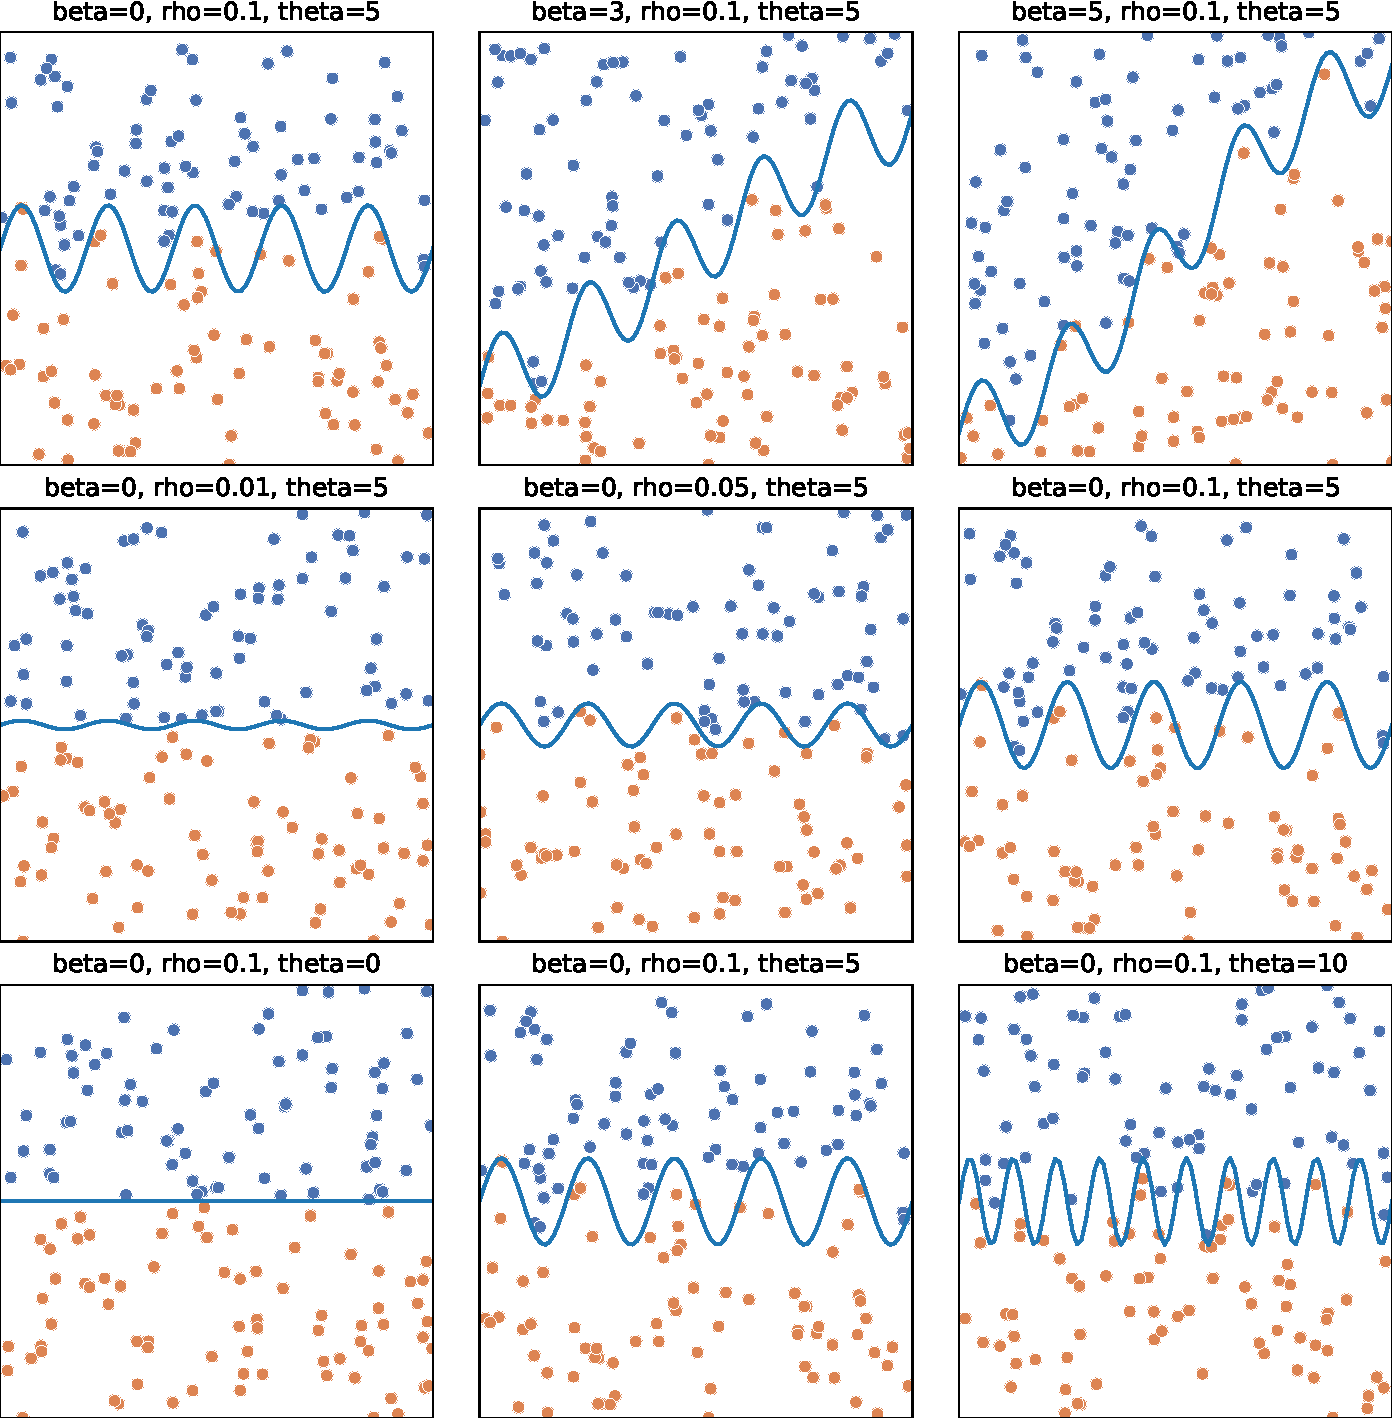
\includegraphics[width=1\linewidth]{img/sinusoid_dataset_param_influence.pdf}
%     \caption{Esempio di dataset generati con funzione sinusoidale. 
%     $\beta$ controlla ?, $\rho$ controlla l'ampiezza, $\theta$ la frequenza.}
%     \label{fig:sinusoid_dataset}
% \end{figure}

\subsubsection{Funzione paraboloide}
% Fissati i parametri $\alpha, x_\text{shift}, y_\text{shift}$, per un vettore $\Vec{x}=\{x_1, \dots, x_n\} \in \mathrm{R}^n$, l'etichetta è calcolata con la funzione
% \begin{equation}\label{eq:pacman_dataset_lf}
% lf(\Vec{x})= x_n - \sum_{i=1}^{n-1}\alpha(x_i - x_\text{shift})^2 - y_\text{shift}.
% \end{equation}
% $\alpha$ controlla l'ampiezza del paraboloide, mentre $x_\text{shift}$ e $y_\text{shift}$ traslano il vertice del paraboloide.
% La~\Cref{fig:pacman_dataset} mostra alcuni esempi di dataset e funzioni di etichettatura al variare dei parametri.

% \begin{figure}[ht]
%     \centering
%     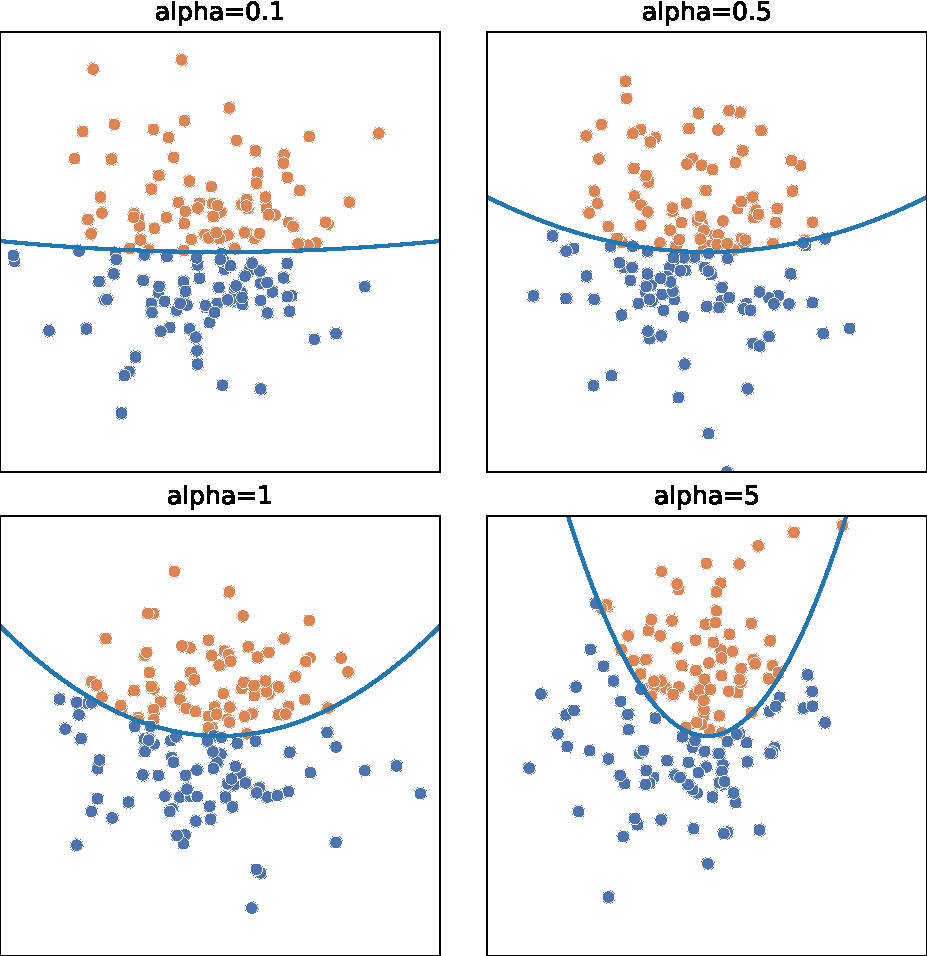
\includegraphics[width=1\linewidth]{img/pacman_dataset_param_influence.pdf}
%     \caption{Esempio di dataset etichettati con paraboloide. $\alpha$ controlla l'ampiezza.}
%     \label{fig:pacman_dataset}
% \end{figure}

% Vengono riportati in~\Cref{tab:parametri_ds_sin,tab:parametri_ds_pacman} i parametri utilizzati per generare i dataset sintetici utilizzati negli esperimenti. Ogni dataset generato con qualsiasi configurazione di parametri è composto da $1000$ elementi: $700$ utilizzati per l'addestramento e $300$ utilizzati esclusivamente per la valutazione dell'accuratezza.
% \begin{table}[h]
%     \centering
%     \begin{tabular}{ccc}
%         \toprule
%         $\beta$ & $\rho$ & $\theta$ \\
%         \midrule
%         0   & 0.01  & 20    \\        
%         0   & 0.025 & 20    \\        
%         0   & 0.05  & 20    \\        
%         0   & 0.075 & 20    \\        
%         0   & 0.1   & 20    \\        
%         95  & 0.2   & 10    \\        
%         0   & 0.1   & 1     \\    
%         0   & 0.1   & 2     \\    
%         0   & 0.1   & 5     \\    
%         0   & 0.1   & 1     \\    
%         \bottomrule
%     \end{tabular}
%     \caption{Configurazioni di parametri utilizzati per generare dataset con la funzione sinusoidale~\Cref{eq:sinusoid_dataset_lf}}
%     \label{tab:parametri_ds_sin}
% \end{table}
% \begin{table}[h]
%     \centering
%     \begin{tabular}{ccc}
%         \toprule
%         $\beta$ & $\rho$ & $\theta$ \\
%         \midrule

%         \bottomrule
%     \end{tabular}
%     \caption{Configurazioni di parametri utilizzati per generare dataset con la funzione paraboloide~\Cref{eq:pacman_dataset_lf}}
%     \label{tab:parametri_ds_pacman}
% \end{table}


\subsection{Dataset reali}
% I dataset reali utilizzati per alcuni esperimenti sono estratti da \emph{UCI Machine Learning repository}~\cite{UCI_ML_repository}. In particolare son state utilizzate delle versioni pre-elaborate e rese disponibili \emph{on-line}\footnote{\url{https://www.csie.ntu.edu.tw/~cjlin/libsvmtools/datasets/binary.html}} in formato LibSVM~\cite{libsvm}.
% Vengono riportate nella~\Cref{tab:uci_datasets} le caratteristiche dei dataset utilizzati.


% \begin{table}[h]
%     \centering
%     \begin{tabular}{cccc}
%         \toprule
%         Nome & Num. dati train & Num. dati test & Num. feature\\
%         \midrule
%         a1a & 1,605	& 30,956 & 123\\
%         a2a & 2,265	& 30,296 & 123\\
%         a3a & 3,185	& 29,376 & 123\\
%         \bottomrule
%     \end{tabular}
%     \caption{Caratteristiche dataset UCI.}
%     \label{tab:uci_datasets}
% \end{table}

\section{Esperiment su dataset sintetici 2D}

\subsection{Esperimenti su dataset con rumore}

\section{Esperiment su dataset sintetici 3D}

\section{Esperiment su dataset reali}

\section{Comparazione con altri metodi}\label{sec:comparazione_metodi}
% Per meglio inquadrare i risultati ottenuti dal metodo proposto in questa tesi, sono state confrontate altre implementazioni di metodi presenti in letteratura. **vfdlk jbstlrsfcnkvbhngsldaa+**

\subsubsection{NSSVM}

\subsubsection{Budgeted Stochastic Gradient Descent}

\subsubsection{IRWLS}












